\documentclass[11pt]{article}
\usepackage[T1]{fontenc}
\usepackage[utf8]{inputenc}
\usepackage{lmodern,amsmath,amssymb,graphicx,geometry,microtype,setspace,booktabs,caption}
\usepackage[hidelinks]{hyperref}
\geometry{letterpaper,margin=1in}
\setlength{\parindent}{0pt}
\setlength{\parskip}{0.55em}
\setlength{\emergencystretch}{2em}
\captionsetup{labelfont=bf,font=small}
\renewcommand{\refname}{References}

\pagestyle{empty}
\renewcommand{\thefigure}{S\arabic{figure}}
\setcounter{figure}{9}

\begin{document}
\begin{figure}[!ht]\centering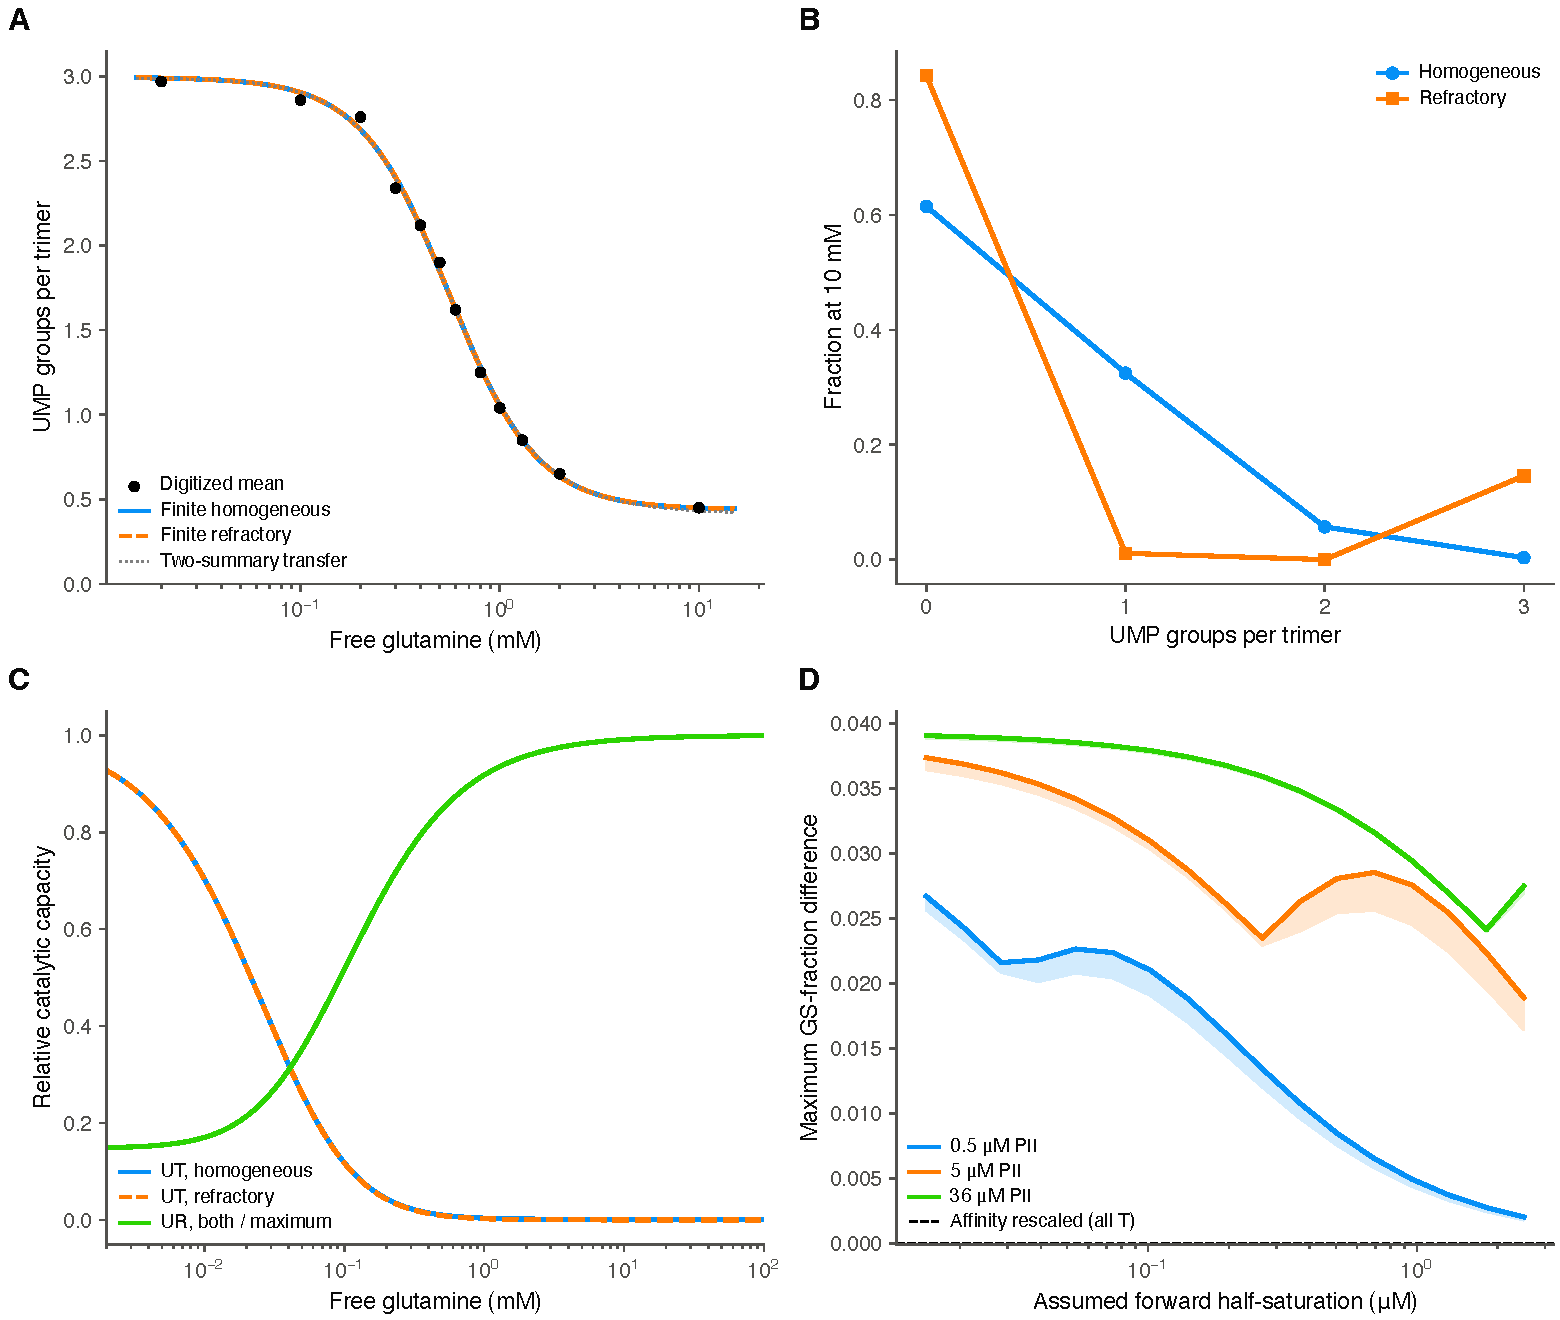
\includegraphics[width=\textwidth,height=0.62\textheight,keepaspectratio]{figure_inputs/FigS10_finite_population.pdf}\begin{singlespace}\caption{\textbf{Finite population alternatives and affinity-rescaling scenarios.} The prior finite homogeneous/refractory comparison is retained with S18--S19. (A) Mean fits. (B) Distinct PII state predictions. (C) Reduced catalytic capacities. (D) Fixed-affinity saturation can distinguish the populations, whereas rescaling an unknown forward affinity restores the stipulated occupancy equivalence. The binding and kinetic assumptions differ from the six-state GlnE development in main Fig 8.}\end{singlespace}\end{figure}
\end{document}
